
%% This is file `talkpal-doc.tex',
%%
%%%%%%%%%%%%%%%%%%%%%%%%%%%%%%%%%%%%%%%%%%%%%%%%%%%%%%%%%%%%
%%
%%  This file is part of the package TALKPAL 1.0, containing 
%%  a style file and its manual which can be used for producing slides
%%  appropriate for a presentation.
%%
%%  Copyright (C) 2026 Palash Baran Pal 
%%  e-mail: palashbaran.pal.retd@saha.ac.in
%%  internet: palashbaranpal.github.io
%%
%%  Release date: July 2026
%%
%%  This program is free software; you can redistribute it and/or modify
%%  it under the terms of the GNU General Public License as published by
%%  the Free Software Foundation; either version 2 of the License, or
%%  (at your option) any later version.
%%
%%  This program is distributed in the hope that it will be useful,
%%  but WITHOUT ANY WARRANTY; without even the implied warranty of
%%  MERCHANTABILITY or FITNESS FOR A PARTICULAR PURPOSE.  See the
%%  GNU General Public License for more details.
%%
%%%%%%%%%%%%%%%%%%%%%%%%%%%%%%%%%%%%%%%%%%%%%%%%%%%%%%%%%%%%%%%
%% Permission is granted to copy this file to another file with a 
%% clearly different name and to customize the declarations in that 
%% copy to serve the needs of your installation.
%% 
%% However, NO PERMISSION is granted to generate or to distribute a 
%% modified version of this file under its original name. 
%% 
%% You are NOT ALLOWED to change this file. 
%% 
%% 

\documentclass[12pt]{article}

%\usepackage{url,multirow, multicol}
\usepackage{euler}
\usepackage{talkpal}

\definecolor{cyan}{rgb}{0,1,1}
\definecolor{leaf}{rgb}{.6,1,.6}
\definecolor{pink}{rgb}{1,.7,.7}
\definecolor{darkblue}{rgb}{0,0,.5}
\definecolor{darkgreen}{rgb}{0,.2,0}
\definecolor{darkred}{rgb}{0.3,0,0}
\definecolor{darkmagenta}{rgb}{0.2,0,0.2}
\definecolor{lightmagenta}{cmyk}{0,0.7,0,0}

\setlength\arraycolsep{15mm}
\parskip=2mm

\def\emph#1{\textcolor{leaf}{#1}}

\def\talkpal{
\raise.01ex\hbox{\textcolor{cyan}{t}}%
\raise-.1ex\hbox{\textcolor{cyan}{a}}%
\raise-.2ex\hbox{\textcolor{cyan}{l}}%
\raise-.3ex\hbox{\textcolor{cyan}{k}}%
\raise-.3ex\hbox{\textcolor{pink}{p}}%
\raise-.15ex\hbox{\textcolor{pink}{a}}%
\raise-.01ex\hbox{\textcolor{pink}{l}}%
}

\def\commcolor{pink}
\def\ecommcolor{green}
\def\ecomm#1{\textcolor{green}{\bf \textbackslash#1}}
\def\noncomm#1{{\textcolor{green}{\bf #1}}}
\def\comm#1{\textcolor{\commcolor}{\bf \textbackslash#1}}
\def\var#1{\textcolor{lightmagenta}{\bf{\em #1}}}
\def\button{{\fboxrule=.5mm\framebox{$\bullet$}}}
\def\file#1{\textcolor{white}{\bf #1}}
\def\txtem#1{\texttt{\sl `#1'}}


\font\titlefont=cmbx10 scaled 6000
\font\ergofont=cmbx10 scaled 2400

\def\section#1{
\fcolorbox{leaf}{red}{
  \textcolor{white}{\Huge #1\vphantom{y}}}}


\def\subsection#1{\ifnum\thensegment>\thecurrlap
  \null \else
  \fcolorbox{yellow}{cyan}{\textcolor{blue}{\LARGE
      #1:}}\fi}

\def\source#1{\rightline{\normalsize\bf{\url {#1}}}}
\def\ergo#1{\null\par \newsegment
  \centerline{\textcolor{cyan}{\ergofont #1}}} 

\def\Item#1{\item[\textcolor{pink}{\bf #1:}]}

\newenvironment{Quote}{\vspace{-5mm}\begin{quote}}{\end{quote}\vspace{-5mm}}


\raggedright

\begin{document}

\begin{center} 

  \textcolor{cyan}{\titlefont \talkpal} 

  \vspace*{0.3\textheight} 

  {\Large A \LaTeX-based presentation software created by}\\[5mm]
  \emph{\Huge Palash Baran Pal}

\end{center}


\beginslide

\section{What the package can do}

The package \talkpal\ is a \LaTeX-based style
file which allows you to create a pdf file with the following
characteristics: 
%%
\begin{enumerate}
  \item Using a multi-media projector, you can project your talk on the
    screen in different slides.

\item The slides can be divided into different segments which can appear
  one at a time, at the push of one key on the keyboard or one click of
  the mouse.

\item You can also use hyperlinks to flash a different portion of the
  file, and come back to the original place.
 
\end{enumerate}

\endslide


\beginslide

\section{The package}

The distribution contains the following files:

\begin{Quote}
\file{manual.tex} \\
\file{manual.pdf} \\
\file{talkpal.sty} \\
\file{slidekey.pl} \\
\end{Quote}

The \file{.sty} file is the style file that will be needed for preparing
presentations.  The \file{.pdf} file is the one you are looking at now,
which helps you understand how the \file{.sty} file works.  The
\file{.tex} was used to create the \file{.pdf} file, and you will not
need it unless you want to see the input commands.  The \file{.pl} file
is a keyboard shortcut explained in the homepage of \talkpal.

\endslide


\beginslide

Since you are reading a PDF file in a PDF viewer software, I will assume
that:
%%
\begin{itemize}

  \item You know how to navigate in a PDF file.  For example, you know
    how to go to the next page or the previous page in a file.  

  \item You know how to use the full screen view.  This is essential for
    giving presentations produced by this software. For viewing this
    file privately, it is not essential except in places where
    hyperlinks are described and used.
    

\end{itemize}

\endslide

\beginslide

\section{Notation used in this manual}

Here are some notations used in writing this file.
%%
\vspace*{-5mm}
\begin{enumerate}\itemsep=-2pt

\item The key (or keys, from the keyboard or from the mouse) used for
  going to the next page will be denoted by \button.

\item Names of pre-existing files and packages appear in \file{this
  color.} 
  
\item Commands defined in standard \LaTeX\ or in pre-existing packages
  will appear in \textcolor{\ecommcolor}{\bf this color}.  So will bash
  commands like \noncomm{latex}.

\item Special \talkpal\ commands will appear in
  \textcolor{\commcolor}{\bf this color}. 

\item Any variable name will appear \var{in this font and color}.  You
  need to put an acceptable name there.  For example, if you see
  \var{colorname}, you might put \emph{red} or \emph{blue}, but not
  \emph{Newton}.
%%%%%
\end{enumerate}
%%
\vspace{-3mm}
Okay, now use \button\  to go to the next slide.


\endslide


\beginslide

\section{\talkpal\ vis-\`a-vis other similar softwares}

I have not used all presentation softwares mentioned here, so my
comments are based on what I heard from others.

Like other softwares with similar objective, \talkpal\ can show the text
in slides and segments, using keyboard buttons to move from one to
another.

It cannot use animation like \file{Power Point} does.  On the other
hand, you can use the rich formatting features of \LaTeX, including
equations and tables etc.  Other \LaTeX-based programs like
\file{beamer} are presumably more elaborate, but they are also much more
complicated.  They have to use separate document classes, so that input
files are very different from ordinary \LaTeX\ files.  On the other
hand, \talkpal, based on the \file{article} class and a style file whose
size is less than 3\,kb, can do most of the things that are necessary
for giving a talk.

\endslide


\beginslide

Some time ago, I created another presentation software called
\file{pptalk}.  The present \talkpal\ is very similar to that one.  The
main difference is that \talkpal\ uses \noncomm{pdf{l}atex} to produce a
\file{pdf} file directly, whereas the earlier program used
\noncomm{latex} followed by \noncomm{dvips} to produce a \file{ps} file
which could then be converted to a pdf file.  The pros and cons of these
two options need not be discussed here.  Since more people use
\noncomm{pdf{l}atex} these days, it seems that \talkpal\ will be more
useful. 


\endslide


\beginslide

\section{How to use \talkpal}
%

First, you need to create the \LaTeX\ file following the instructions
given later in this document.  

Suppose the name of this .tex file is \file{xyz.tex}. Issue the command
%
\begin{Quote}
\noncomm{pdf{l}atex} \quad \var{xyz}
\end{Quote}
%
from your terminal or the pull-down menu on your editor.  This produces
a file called \file{xyz.pdf}.  Open it on your computer screen using any
standard pdf reader and project it by using the hardware available for
that.

\newsegment
\bigskip

The rest of this manual describes how to create the input \file{.tex}
file that is necessary for the procedure.\label{p:endblack}

\endslide

\setbasecolor{darkblue}

\beginslide

\section{How to organize the file}

You don't need to use a new class file in order to write your talk
with \talkpal.   You can use the \noncomm{article} class file.  Use the
package \talkpal.  In other words, start your file as follows:
%
\begin{Quote}
\ecomm{documentclass[12pt]\{article\}} \\ 
\ecomm{usepackage\{talkpal\}}
\end{Quote}
%
and of course, with the commands for beginning and ending the document.
In the middle, you can write \LaTeX\ in the usual way, i.e., as one does
for writing a paper. On running \ecomm{pdf{l}atex}, you will then obtain a
file which will be presentable.  In this case, \talkpal\ merely fixes
the size of the pages.  You can force pagebreaks at suitable points by
using the \ecomm{newpage} command.

However, with \talkpal, you can do much more, as described below.

\endslide

\beginslide

A few pieces of recommendation:

\begin{itemize}\itemsep=0pt
\item \underline{Be careful} to include the \noncomm{12pt} option in the
\ecomm{documentclass} declaration, as shown above.  The sizes of fonts
have been set with this option in such a way that appears nice on the
projected screen.

\item \underline{Do not use} any of the page style commands like
\ecomm{textheight} or \ecomm{textwidth}.  These have already been set
by \talkpal\ to some optimum values which will suit a screen
presentation.

\item You may include other packages.  But put them before the
\talkpal\ package so that nothing in \talkpal\ is overridden by them.


\end{itemize}
\endslide



\beginslide

\section{Some ``don'ts''}
\begin{itemize}\itemsep=0pt

  \item \underline{Do not include} the following packages in your .tex
    file, because they are already included in \talkpal:
    \begin{center}
    \begin{tabular}{l@{\quad\quad}l@{\quad\quad}l}
      \file{color} & \file{graphicx} & \file{lastpage} \\
      \file{newcent} & \file{fancyhdr} &  \file{hyperref}
    \end{tabular}
    \end{center}
    
\item Do not get turned off by the use of colors in this manual.  Some
  of them, like the main font color, are defaults, but you can change
  them by commands shown later.  Some others are defined within this
  document and have nothing to do with the style file for \talkpal, like
  the colors in section headings and in displaying different commands.
  You can check the file \file{manual.tex} to find what has been defined
  there.

\end{itemize}


\endslide



\beginslide

\section{Dividing text into slides}

You need to decide how much (or how little) of text you want to put in
a particular slide.  When you want to begin the slide, type

\begin{Quote}
\comm{beginslide}
\end{Quote}

Then continue with whatever you want to put there, typing things just
as in a normal \LaTeX\ file.  

Divide things into paragraphs as you want, put text and equations as
necessary.  When you finish typing the contents of the slide, type
%
\begin{Quote}
\comm{endslide}
\end{Quote}
%
After that,  use the \comm{beginslide} command to start a new slide.

If you put too much in a slide, text will spill at the bottom of the
slide.  You need to reconsider where to end the slide.


\endslide


\beginslide

\section{Dividing slides into segments}

For a presentation, it is best to unfold the contents of a page in a
number of segments, one segment appearing at a time.  This way, the
members of the audience are not exposed to a flurry of material at a
time.

For this, start writing the slide with the first segment, after the
\comm{beginslide} command.  When you want to start the next segment,
just type
%
\begin{Quote}
\comm{newsegment}
\end{Quote}
%
and then write the text for the next segment.  Continue this process,
adding more segments if you want, until you reach the end of the slide
with \comm{endslide}.

\endslide

\beginslide

Let us see an example.  Notice that there is a huge empty portion
at the bottom of this slide.  This is because there are more segments
down there which are hidden.  Use \button\  now.



\newsegment

\textcolor{leaf}{Now you see the next segment!}  You can continue this
way, introducing more segments.  In principle, the number of segments
on a page can be unlimited.  However, the height of the page and the
size of the font introduces some obvious restrictions.

Want to see more on this page? Hit \button.

\newsegment


{}From now on, hit \button\  whenever you want to see some more
material on the screen: whether material continued on the same slide
or on a different slide.

\endslide

\beginslide

You can put the command \comm{newsegment} almost anywhere in the file.
You can put it at the end of any paragraph, as we have done once or
twice earlier and will do more often from now on.

\newsegment

But the command can also be put in the middle of a paragraph, as you
will find out if you hit \button\  now. \newsegment You can put
the command before or after an equation, before or after a table, or
even in the middle of a word like (let's see if I can spell it right)
\textcolor{red}{ ``super\-\newsegment calli\newsegment fragi\newsegment
  listic\newsegment expi\newsegment alli\newsegment docious''.}

\endslide


\beginslide


You can also put the command within groups.  By \noncomm{group}, I mean
anything which is between a matching \ecomm{begin} and \ecomm{end} pair,
or a \ecomm{left}-\ecomm{right} pair in math mode.  It can be a table,
an environment like quote or enumerate, an equation, part of math mode
which uses matching brackets.

\newsegment

However, in this case you will have to do a bit more.  The
command \comm{newsegment} works only within a group.  So, when the
group ends, if you want to continue with the same segment, put the
command 
%
\begin{Quote}
\comm{samesegment}
\end{Quote}
%
and keep writing.

\endslide


\beginslide


For example, in writing
%
\begin{eqnarray*}
x =  \newsegment 
\pmatrix{x_1 \cr x_2} \,,
%\label{}
\end{eqnarray*}
%
\samesegment 
I had to put the \comm{samesegment} command at the end of
the equation. \newsegment  And when I wrote  
%
\begin{eqnarray*}
x = \left[ \frac1a + \newsegment \frac1b \right] \samesegment (y+2) 
%\label{}
\end{eqnarray*}
%
\samesegment using \ecomm{left[}$\cdots$\ecomm{right]}, 
I had to put the \comm{samesegment} command after
the closing square bracket.\label{p:endblue}


\endslide


\beginslide

\section{Vertical segmentation}

The \comm{newsegment} command allows you to make horizontal segments.
If you want vertical  segments, you should use the \noncomm{minipage}
environment for that.  See an example here:

\newsegment

%%
\begin{center}
\begin{minipage}{0.3\textwidth}
This is the first segment, which can contain anything you like.  Hit
\button\ to see the next segment.
\end{minipage}
%%
\hfill\newsegment
%%
\begin{minipage}{0.3\textwidth}
This is the second segment.  Again hit \button\ to see the third and
last segment.
\end{minipage}
%%
\hfill\newsegment
%%
\begin{minipage}{0.3\textwidth}
  Using too many vertical segments will make the segments narrow,
  which would not look good.
\end{minipage}
\end{center}
%%
\samesegment
\newsegment

\bigskip

To see how this has been produced, hit \button\ to go to the next slide.


\endslide 


\beginslide

%%
\begin{center}
\begin{minipage}{0.3\textwidth}
The right panel shows the commands which produced the vertical
segmentation in the previous slide.  \emph{Note that} one cannot leave
blank lines between minipages, because that would result in the
minipages occurring in different paragraphs.
\end{minipage}
%%
\hfill
%%
\begin{minipage}{0.4\textwidth}
  \putfigure{0.9\textheight}{}{vertseg.png}
\end{minipage}
\end{center}
%%


\endslide 



\setbasecolor{darkmagenta}

\beginslide

\section{How to use colors}

You have already seen colors being used in this sample file.  This has
been done by using the package \file{color}.  \talkpal\ itself has this
package as an input, so you should not introduce it explicitly when
you are using \talkpal.


\newsegment

The \file{color} package defines two commands for implementing colored
text.  One of them is \ecomm{textcolor}, used for a local change of
color.  The syntax is
%
\begin{Quote}
\ecomm{textcolor}\var{\{{colorname}\}\{Text material\}}
\end{Quote}
%
which makes the \txtem{`Text material'} to appear in the color given
as \txtem{`colorname'}.  This command has been suitably redefined in
\talkpal, and will work exactly the same way within \talkpal.

\endslide


\beginslide

On the other hand, you can use the command
%
\begin{Quote}
\ecomm{color\{\var{colorname}\}}
\end{Quote}
%
which is a declaration valid for the rest of the document.

If you use it at the beginning of your document or between two slides
(i.e., after an \comm{endslide} and before the next \comm{beginslide}),
the change will affect the rest of the document. \color{white} If you
use it within a slide (as it has been done at the beginning of this
sentence), it will work only until the end of the slide.  You will see
the normal textcolor returning when you go to the next slide.


\endslide


\beginslide

\section{Color names}

The basic color names appear in the file \file{color.sty}, which is part
of the color package.  They are: \emph{red, blue, green, cyan, magenta,
  yellow}, and the non-colors \emph{white and black}.

\newsegment

You can also create new colors.  For example, a color called \var{RONG}
can be defined by any of the following commands, where each $p_i$ is a
number between 0 and 1:
%
\begin{Quote}
\ecomm{definecolor\{\var{RONG}\}\{rgb\}\{\var{$p_1,p_2,p_3$}\}} 
\ecomm{definecolor\{\var{RONG}\}\{cmyk\}\{\var{$p_1,p_2,p_3,p_4$}\}}  
\ecomm{definecolor\{\var{RONG}\}\{gray\}\{\var{$p_1$}\}}
\label{p:newcolors}
\end{Quote} 
%
The last command produces only shades of gray.  Try these out.\label{p:endblue}

\endslide


\beginslide

\section{Background color}

You have probably noticed that the background color of the slides
changed after Slide~\pageref{p:endblack}.

It changed to a dark blue, because the command

\begin{Quote}
\comm{setbasecolor\{darkblue\}}
\end{Quote}

was issued before the \comm{beginslide} corresponding to that slide.
The color \emph{darkblue} has been defined by the command
%
\begin{Quote}
\ecomm{definecolor\{darkblue\}\{rgb\}\{0,0,0.5\}}
\end{Quote}
%
as explained earlier on Slide~\pageref{p:newcolors}.  This change is not
part of the \talkpal\ style file.  It has been used in this manual file,
to give examples of how you can change colors.  Look out for the next
change in the base color.

\endslide

\beginslide

\section{Suggestions on colors}

I have a few recommendations on the use of colors.  None of these is
binding. 
%%
\vspace{-5mm}
\begin{enumerate}\topsep=-40pt\itemsep=0pt
%
\item Use your judgement for color contrasts.  Needless to say, the
contents of a slide will not be very legible if you use orange letters
on a yellow background.

\item Use dark backgrounds and light-colored text for best results.
  Light-colored backgrounds put unnecessary and bothersome glare on the
  eyes of the people in the audience.

\item It is best not to define a new color unless you absolutely need
  to do so.  But if you need to, there is no restriction.

\item Background colors may be changed while moving from one section of
  the talk to the next.  That's what I have done in this document.
  

\end{enumerate}
%%

\endslide

\setbasecolor{darkgreen}

\beginslide

\section{Math mode}

You can use math mode in much the same way that you use it for a usual
\LaTeX\ document, keeping the following recommendations in mind:
%%
\begin{enumerate}

  \item Normal math mode font for \LaTeX\ is too thin, and does not look
    very good on slides.  I advise using \ecomm{usepackage\{euler\}} in
    the preamble of your file.  I have used it for producing this
    document.

  \item Do NOT cross-refer equations by putting labels if you use
    multiple segments in a slide.  I am against labeling and
    cross-referencing anywhere, because it is useless to say something
    like ``...as shown in Eq. (17) earlier...'' during a talk.  So,
    for displayed equations, use either the \noncomm{eqnarray*}
    environment, or use delimiters \noncomm{\$\$} at both ends.
    

\end{enumerate}

\endslide


\beginslide

\section{Displaying figures}

Figures are included by the command \ecomm{includegraphics}.  The file
\file{graphicx.sty} is included in \file{talkpal.sty}, so you should not
ask your \file{.tex} file to include it again.

If the \ecomm{includegraphics} command does not appear in the first
segment of a slide, you need to hide your picture until the proper
segment arrives.  For this, you need a slightly modified command:

\begin{Quote}
\comm{putfigure\{\var{pictureheight}\}\{\var{other size
    commands}\}\{\var{filename}\}}
\end{Quote}

The middle part can be empty.  But the declaration of the height is
essential, for which the amount should be specified without
\ecomm{height=}.  Examples:

\begin{Quote}
\comm{putfigure\{\noncomm{0.3}\ecomm{textheight}\}
  \{\noncomm{width=0.7}\ecomm{textwidth}\}\{\var{parabola.png}\}} \\ 
\comm{putfigure\{\var{5cm}\}
  \{\}\{\var{parabola.png}\}} \\ 
\end{Quote}
%%

\endslide

\beginslide

Do \emph{NOT} put the figure in a \file{figure} environment, i.e.,
something starting with \ecomm{begin\{figure\}} and ending with
\ecomm{end\{figure\}}.  The \file{figure} environment turns the figure
into a floating object, and \LaTeX\ decides where to put it.  Just for
creating the figure, the \ecomm{includegraphics} is good enough, as
modified here in \comm{putfigure}.

\newsegment

Here is an example of what \comm{putfigure} can do:
%%
\putfigure{0.2\textheight}{}{parabola.png}

\newsegment

If you want to put multiple pictures side by side, use \file{minipage}
environments, as discussed earlier in the section on ``Vertical
segmentation''.
\begin{center}
\begin{minipage}{0.2\textwidth}
\putfigure{0.2\textheight}{}{parabola.png}
\end{minipage}
\hspace{2cm}
\begin{minipage}{0.2\textwidth}
\putfigure{0.2\textheight}{width=0.3\textwidth}{parabola.png}
\end{minipage}
\end{center}

\endslide

\beginslide

\section{Tables and other floats}

For reasons mentioned in connection with figures, do not use the
\noncomm{table} environment that \LaTeX\ provides.  The same applies to
all environments that put some stuff as float.

\newsegment

\vspace{-3mm}
\begin{center}
  \begin{tabular}{c|cc}
    A & B & C \\  
    \hline 
    D & E & F \\  
    G & H & I
  \end{tabular}
\end{center}
\vspace{-3mm}

Just for creating a table (an example given above), the
\noncomm{tabular} environment is good enough.  If the entries contain
too many math symbols, you can also use the \noncomm{array} environment,
putting the table within an equation.

\newsegment

Do not put the \comm{newsegment} command within a table.

\endslide

\beginslide

\section{Using \noncomm{hyperref}}

As said before, cross-referencing is a bad idea.  If you must want to
refer to something mentioned elsewhere in the document, use 
\noncomm{hyperref} commands.  This package is also included in \talkpal,
so you must not include it again.

\newsegment

Hyperref commands appear in pairs.  At the source, use the command
%%
\begin{Quote}
  \comm{hyperpair\{\var{AAA}\}\{\var{BBB}\}}
\end{Quote}
%%
where the variables are labels of your choice.  At the target, put the
same command, with the same labels in opposite order, i.e., 
%%
\begin{Quote}
  \comm{hyperpair\{\var{BBB}\}\{\var{AAA}\}}
\end{Quote}
%%
This way, you will get two arrows, one at the source and one at the
target.  If you click on them, you can go back and forth.
%%
\newsegment
%%
Check it by pressing on this arrow\hyperpair{sourcearrow}{targetarrow}
to go to the last page, and press the arrow there to come back here.

\endslide

\beginslide

You may also put an optional argument in the command \comm{hyperpair},
which will appear as the symbol for the hyperref spot.  This argument
can be different for the source and the target, if you wish.  Here is an
example of how to do it:
%%
\begin{Quote}
  \comm{hyperpair[\comm{spadesuit}]\{\var{BBB}\}\{\var{AAA}\}}
\end{Quote}
%%

Try using it for going to a certain place near the end of this
document.\hyperpair[$\spadesuit$a]{ss}{tt}

\newsegment

\bigskip\bigskip

\framebox {Warning:} Hyperlinks do not work properly unless the full-screen view is
used. 

\endslide

\beginslide

\section{Flashing}


You might also want to flash a picture or a big formula, but do not want
to carry it in the rest of your slide.  This can be done by putting the
object in a picture file such as \file{flashpic.png}, and then issuing a
command like this:

\comm{flash\{\var{0.2}\}
  \{\ecomm{includegraphics}[\noncomm{height=0.8}\ecomm{textheight}]\{\var{flashpic.png}\}\}}

The first argument raises the flashed object by that fraction of
\ecomm{textheight}.  The second argument is the object to be flashed.

\newsegment

Try hitting \button\  here to see such a flash appear, and hit it again
after you will have seen the flashed material.

\flash{0.6}{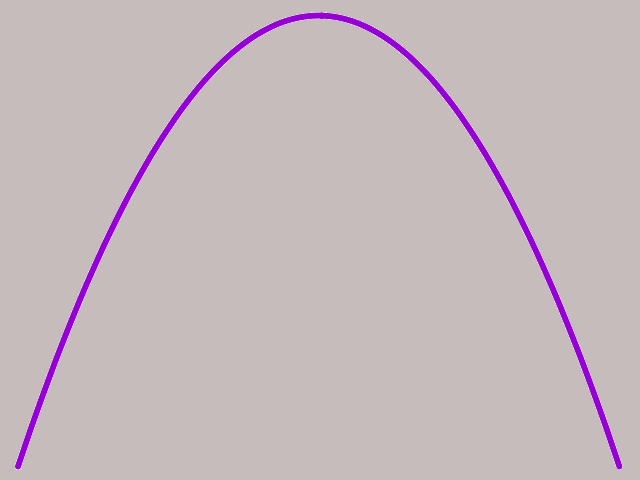
\includegraphics[height=0.8\textheight, width=0.9\textwidth]{parabola.png}}


\newsegment

\bigskip\bigskip

You have arrived at the next segment, where the ``flash''ed component
has disappeared.


\endslide

\beginslide

\section{On defaults, and how to change them}

The default font family for \LaTeX\ is \noncomm{cmr}.  These fonts are
not suitable for slide presentations.  So I have reset the default to
\noncomm{newcent}.  The \noncomm{palatino} and the \noncomm{times}
families also work quite well.  If you want to use \noncomm{palatino},
for example, put the command
%
\begin{Quote}
\ecomm{usepackage\{palatino\}}
\end{Quote}
%
For \noncomm{helvetica}, I don't know whether there is a
similar package, but you can use the command
%
\begin{Quote}
\ecomm{renewcommand}\ecomm{familydefault\{\ecomm{sfdefault}\}}
\end{Quote}
%%
Such commands must be put in the preamble of the file after the
\talkpal\ package has been included.

\endslide


\beginslide

Other defaults are summarized in the following table, with examples of
how to change them.
%%
\begin{center}
\begin{tabular}{lll}
\hline
Parameter & Default value & Example of change \\ 
\hline
Font size & \noncomm{Large} & \ecomm{def}\comm{defaultsize}\{large\} \\
Text color & yellow & \ecomm{color}\{white\} \\
Background color & black & \comm{setbasecolor}{\{blue\}} \\
Foottext & Created with talkpal & \ecomm{def}\comm{foottext\{\var{My talk}\}}
\\
Footcolor & white & \ecomm{def}\comm{footcolor}\{pink\}
\\
\hline
\end{tabular}
\end{center}

Please note that some of the commands need a leading \ecomm{def}, while
others do not.

\endslide

\setbasecolor{darkred}

\beginslide

\section{Summary of commands}

Here is a summary of the special commands for \talkpal.
%
\begin{list}{}{\itemsep=0pt}
\item[\comm{beginslide}$\,\cdots\,$\comm{endslide}] Denotes the
beginning and end of a slide.  The contents of the slide goes in the
middle, in place of the three dots.

\item[\comm{newsegment}] Denotes the beginning of a new segment in a
slide.  Not required for the first segment in a slide, which begins
with the \comm{beginslide} declaration.

\item[\comm{samesegment}] If the \comm{newsegment} appears within a
group, this command has to be used at the end of the group to reassert
the continuation of the segment after the group.\hyperpair[$\clubsuit$a]{tt}{ss}

\end{list}

\endslide

\beginslide

%
\begin{list}{}{\itemsep=0pt}
\item[\comm{putfigure}] Necessary for placing figures inside the
  presentation. 

\item[\comm{flash}] Flashes a picture in a particular segment, which
  vanishes when the next segment is activated.  The ``picture'' can be
  anything in a picture file, even a long formula.
  
\item[\comm{setbasecolor}] Changes the background color of slides.

\item[\ecomm{def}\comm{defaultsize}] Defines the default size of text.

\item[\ecomm{def}\comm{foottext}] Changes the foottext.

\item[\ecomm{def}\comm{footcolor}] Changes the color of the material in
  the footer.

\end{list}
%%
As an example, we change the foottext and footcolor after this
slide, with appropriate commands after the \ecomm{endslide} of this
page.

\endslide

\def\foottext{The talkpal manual: written by Palash B. Pal}
\def\footcolor{pink}

\beginslide


It is also useful to master the use of some commands which are not
\talkpal\ specials, but are not used while writing papers and books.
%
\begin{Quote}
\begin{list}{}{\topsep=-1mm}
\item[\ecomm{definecolor}] Used for defining colors.

\item[\ecomm{textcolor}] Redefines the text color locally.

\item[\ecomm{color}] Defines the text color either till the end of the
  slide or till the end of the document, as explained earlier.

\item[\ecomm{pageref}\{Lastpage\}]  Puts the number of the last slide.
  For example, footers in this document have been produced by the
  command
  
  \comm{foottext}\{Created with talkpal \ecomm{hfill} 
  Slide~\ecomm{arabic}\{page\} of \ecomm{pageref}\{LastPage\}\}

\end{list}
\end{Quote}
%%

These commands are defined in the standard packages \file{color} and
\file{lastpage}, both of which are included in
\talkpal.\hyperpair{targetarrow} {sourcearrow}

\endslide

\end{document} 




\beginslide



\endslide



